\graphicspath{{Definitions/Figures/}}

\chapter{Definitions} \label{sec:definitions}

\section{Jet}

A jet can be considered as a collimated spray of stable particles that arises from the fragmentation and hadronization of a quark or a gluon \cite{Jets}. Since a jet is a shower of particles, algorithms of reconstruction have to be defined to gather all the information from the shower and define a jet as single element observed in the detector. The most common algorithms that define jets assume that the particle shower will arrive in a conical region in the detector. Hence, these algorithms establish a cluster in the $\eta-\phi$ space that defines where all the particles that make up the jet would arrive.

A schematic description of the production and definition of a jet is presented in Figure \ref{fig: jet diagram}. The diagram shows how, as a result from the proton-proton collision, gluons and quarks are generated. Then, as described later in Section \ref{sec: simulation}, the partons hadronize resulting in stable particles that are then observed in the detector. It can be seen in the figure the importance of defining correctly the cone of the jet. If the cone radius is too small, some particles that came from the initial parton may be left out, but if the radius is too large some particles that came from a different parton can be mistaken as part of the jet.

\begin{figure}[H]
\centering
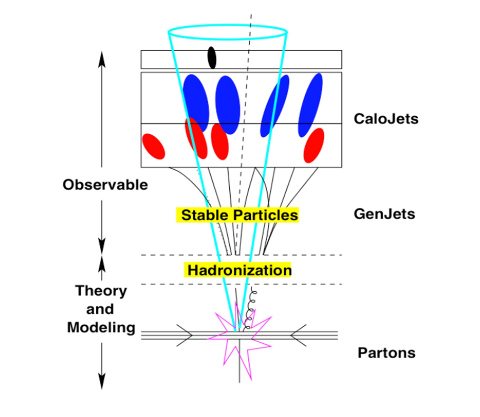
\includegraphics[width = 0.7\linewidth]{jetsDiagram}
\caption{Schematic diagram of the creation and definition of a jet. (Taken from \cite{Jets})}
\label{fig: jet diagram}
\end{figure}

Variations of the cone algorithms are defined to gain more precision in the jet definition. Being able to reconstruct correctly all the particles making up the jet is important, because the jet provides a link between the observed particles in the detector and the physics at the partonic level \cite{Jets}. In other words, since gluons and quarks decay rapidly, the only way to obtain information in detectors about processes related to partons are through jets. This is why more sophisticated algorithms to fully reconstruct jets in detectors and simulations are developed. For example, the iterative cone with progressive removal algorithm, or IC-PR algorithm, is used in CMS and the software Pythia \cite{Jets}. The algorithm starts by finding the cell in the detector with largest transverse momentum and makes it a seed. Then, a cone is defined around the seed and a trial jet axis is calculated. If the trial jet axis is the same as the axis of the cone defined from the seed, then the cone is labelled as stable and all the particles that lie inside the cone are defined as the jet. If the trial jet axis does not equal the seed axis, the trial jet axis is defined as the new seed axis. The process described above is repeated until a convergence of the axes occurs. This algorithm is repeated until there are no seeds above a threshold energy left \cite{Jets}.  


\section{Variable Definitions}

The transverse momentum or $p_{T}$, is defined as the momentum component that a particle has in the plane perpendicular to the beam line. In the coordinate system of the LHC, the transverse plane corresponds to the $x-y$ plane.

The variable related with the polar angle in the LHC is called pseudorapidity, or $\eta$, defined as in Equation \ref{eq: eta}. The use of this variable is justified for mainly two reasons. The first one is that $\Delta \eta$, contrary to $\Delta \theta$, is a Lorentz invariant. This makes $\Delta \eta$ a more natural variable than $\Delta \theta$ for relativistic calculations. The second reason is that the distribution of the values of $\eta$ in the barrel region, where the multiplicity of particle is less than in the end-caps, is wider, allowing $\eta$ to have a more uniform particle number distribution.

\begin{equation}
 \eta = -\ln\left[\tan\left(\frac{\theta}{2}\right)\right]
 \label{eq: eta}
\end{equation}

Sometimes it is necessary to determine the total angular separation between two particle in the detector, that is, determining the separation in both $\phi$ and $\eta$. This is accomplished using the variable $\Delta R$, defined in Equation \ref{eq: deltaR}. As stated earlier, it is generally used to determine how close in the detector two particles are. Taking this into account, $\Delta R$ is useful to establish whether two particles may have overlapped detection points in the detector. 

\begin{equation}\label{eq: deltaR}
\Delta R = \sqrt{\left(\Delta \eta\right)^{2} + \left(\Delta \phi \right)^{2}}
\end{equation}

Another useful variable defined in particle physics is the missing transverse energy or $\slashed{E}_{T}$. Given that the protons in the LHC collide along the $z$ axis, the initial momentum in the $x$ and $y$ components is zero. Since momentum in all directions must be conserved during the collision, the momentum after the collision must also be zero. However, there are particles resulting from the proton-proton collision, such as the neutrinos, that cannot be observed by the components in the detector. That is why the energy corresponding to these unobserved particles is going to be missing from the energy observed in the detector. Considering what has been said in this paragraph, the momentum equation in the $x-y$ plane must be

$$ \sum_{i=1}^{m} p_{T}(i)^{observed} + \sum_{j=1}^{n} p_{T}(i)^{missing} = 0 $$

Taking the last equation into account, it is natural to define the missing transverse energy as the negative sum of transverse momenta of the observed particles in the detector. This definition is presented in Equation \ref{eq: MET}.

\begin{equation}\label{eq: MET}
\slashed{E}_{T} = -\sum_{i=1}^{m} p_{T}(i)^{observed}
\end{equation}  



With the idea of exploiting the possible difference between signal and background in the $p_{T}$ for jets and $\tau$'s, two new variables shown in Equations \ref{eq: HT} and \ref{eq: ST} were defined to check for possible further separation between signal and background. As shown in equation \ref{eq: HT}, the $H_{T}$ variable is defined as the scalar sum of the jets in the event that are not B-jets. $S_{T}$ is defined as the scalar sum of jets that fullfilll the same conditions of $H_{T}$, added to the $p_{T}$ of the $\tau$'s in the event.


\begin{equation}
 H_{T} = \sum_{i=1}^{n} p_{T}(jet_{i})
 \label{eq: HT}
\end{equation}

\begin{equation}
 S_{T} = \sum_{i=1}^{n} p_{T}(jet_{i}) + \sum_{j=1}^{m} p_{T}(\tau_{j})
 \label{eq: ST}
\end{equation}

Throughout the analysis it is important to establish a cuantitative estimator to define the amount of signal compared to the amount of background. For that purpose, a cuantitative estimator, commonly known as figure of merit, is used to determine optimal cuts in the relevant variables. This figure of merit allows to find the optimal cuts in the relevant variables by giving a cuantitative result of the amount of signal events compared to the number of background events. For this particular analysis, the significance formula that was used is the one shown in Equation \ref{eq: significance}, where $S$ is the significance, $N(s)$ is the number of signal events, and $N(B)$ is the number of background events.

\begin{equation} \label{eq: significance}
    S = \frac{N(s)}{\sqrt{N(s) + N(B)}}
\end{equation}






 



